% Drawing 142/06-5 -- folder 142, batch 06, archive page 105 (PDF page 106).
% Transcription: Cinquième figure. Un seul sommet sur le cercle de $0$, un chemin vers le cercle de $1$ (étiquette raturée), le point $\infty$ isolé ; flèches $\Lambda^+_0$ et $\Lambda^{01}_+$. Légende : « 1 sommet, 2 flèches, 0 relation » ; dessous : « 3 cas. »
% Kind: quiver on the sphere minus three points (small circles and paths). Method 2 (schematic redraw from the facsimile). Status: ok.
% Notes: One vertex on the circle of 0, a doubled path to the circle of 1; infinity isolated in a pencil circle; a pencil loop round the figure. Arrows Lambda^+_0 and Lambda^{01}_+; the label on the path is overinked (struck) and left out. Legends "1 sommet, 2 fleches", "0 relation", "3 cas".
% Coordinates: 1 unit = 1 mm = 1/100 of the crop width (bbox in page fractions: [0.1, 0.38, 0.51, 0.557]).
% Redrawn by Claude (claude-opus-5-5), issue #73, 2026-11-07; not checked by a human; not compiled (no TeX in the session).
% Rights: reproduces part of the work -- behind RENDER_TRANSCRIPTS, never published by itself.
\documentclass[tikz,border=3pt]{standalone}
\usepackage{amsmath,amssymb}
\usetikzlibrary{patterns,arrows.meta}
\tikzset{pencil/.style={black!45}, struck/.style={black!35}, mark/.style={circle,draw,inner sep=1.3pt}, pt/.style={circle,fill,inner sep=0.9pt}, opt/.style={circle,draw,fill=white,inner sep=1.1pt}}
\begin{document}
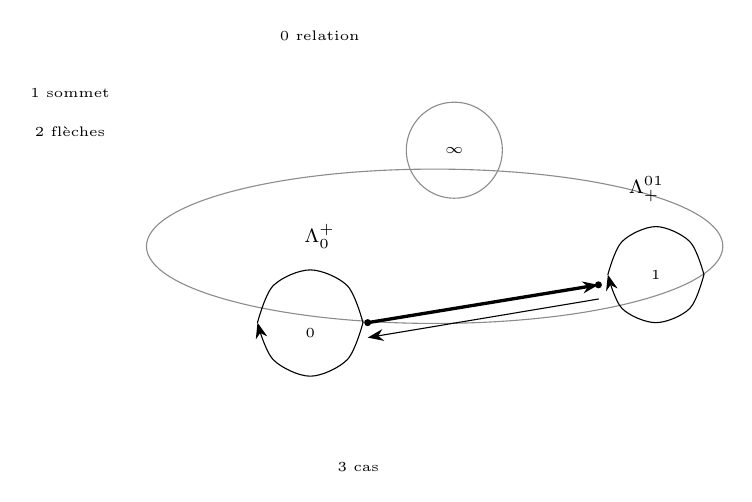
\begin{tikzpicture}[x=1mm,y=1mm,line cap=round,line join=round,font=\scriptsize]
\draw[pencil] (58.5,-30.5) ellipse[x radius=36.6, y radius=9.8];
\draw[pencil] (61,-18.3) circle[radius=6.1];
\node[inner sep=1pt] at (61,-18.3) {\tiny $\infty$};
\draw plot[smooth, tension=0.55] coordinates {(36,-40.2) (38,-35.5) (42.7,-33.5) (47.4,-35.5) (49.4,-40.2)};
\draw[-{Stealth[length=2mm]}] plot[smooth, tension=0.55] coordinates {(49.4,-40.2) (47.4,-44.9) (42.7,-47) (38,-44.9) (36,-40.2)};
\draw plot[smooth, tension=0.55] coordinates {(80.5,-34.1) (82.3,-29.9) (86.6,-28) (90.9,-29.9) (92.7,-34.1)};
\draw[-{Stealth[length=2mm]}] plot[smooth, tension=0.55] coordinates {(92.7,-34.1) (90.9,-38.4) (86.6,-40.2) (82.3,-38.4) (80.5,-34.1)};
\node[pt] at (50,-40.2) {};
\node[pt] at (79.3,-35.4) {};
\draw[-{Stealth[length=2mm]},very thick] (50,-40.2) -- (79.3,-35.4);
\draw[-{Stealth[length=2mm]}] (79.3,-37.2) -- (50,-42.1);
\node[inner sep=1pt] at (42.7,-41.5) {\tiny $0$};
\node[inner sep=1pt] at (86.6,-34.1) {\tiny $1$};
\node[inner sep=1pt] at (43.9,-29.3) {\scriptsize $\Lambda^+_0$};
\node[inner sep=1pt] at (85.4,-23.2) {\scriptsize $\Lambda^{01}_+$};
\node[inner sep=1pt] at (12.2,-11) {\tiny 1 sommet};
\node[inner sep=1pt] at (12.2,-15.9) {\tiny 2 fl\`eches};
\node[inner sep=1pt] at (43.9,-3.7) {\tiny 0 relation};
\node[inner sep=1pt] at (48.8,-58.5) {\tiny 3 cas};
\end{tikzpicture}
\end{document}
